%==========================================================================%
%  Understanding Feature Fusion Strategies in Transformer-based           %
%  Image Restoration: Evidence from Document Shadow Removal               %
%  Target: Applied Intelligence (APIN), Springer                          %
%  Template: Springer Nature sn-article (sn-mathphys-num)                 %
%==========================================================================%

\documentclass[pdflatex,sn-basic,Numbered]{sn-jnl}

%% ---- Numbered references (APIN requirement) ----
\setcitestyle{numbers,square}

%% ---- Standard Packages ----
\usepackage{graphicx}
\usepackage{multirow}
\usepackage{amsmath,amssymb,amsfonts}
\usepackage{amsthm}
\usepackage{mathrsfs}
\usepackage[title]{appendix}
\usepackage{xcolor}
\usepackage{textcomp}
\usepackage{booktabs}
\usepackage{algorithm}
\usepackage{algorithmicx}
\usepackage{algpseudocode}

%% ---- Theorem styles ----
\theoremstyle{thmstyleone}
\newtheorem{theorem}{Theorem}
\newtheorem{proposition}[theorem]{Proposition}

\theoremstyle{thmstyletwo}
\newtheorem{example}{Example}
\newtheorem{remark}{Remark}

\theoremstyle{thmstylethree}
\newtheorem{definition}{Definition}

\raggedbottom

\begin{document}

%% ---- Title ----
\title[Fusion Strategies in Transformer Restoration]{
Understanding Feature Fusion Strategies in Transformer-based Image Restoration: Evidence from Document Shadow Removal
}

%% ---- Authors (to be filled) ----
\author[1]{\fnm{Author} \sur{One}}\email{author1@example.com}
\author[1]{\fnm{Author} \sur{Two}}\email{author2@example.com}
\author[1]{\fnm{Author} \sur{Three}}\email{author3@example.com}

\affil[1]{\orgname{Institution}, \orgaddress{\city{City}, \country{Country}}}

%% ---- Abstract ----
\abstract{
Transformer-based architectures have become the dominant backbone for image restoration, yet a fundamental question remains unanswered: how should auxiliary modality features be fused into these networks? While numerous fusion mechanisms---concatenation, cross-attention, FiLM modulation, gating---have been proposed across different tasks, the absence of controlled comparisons under a unified framework has left the community without evidence-based guidance on fusion strategy selection.
In this paper, we conduct a systematic study of five representative fusion strategies within a controlled Restormer framework across synthetic (SD7K) and real-world (RDD) document shadow removal datasets.
Our investigation reveals three key findings.
First, fusion strategy rankings are \textit{domain-dependent}: FiLM modulation achieves the highest PSNR on synthetic data (24.77~dB), while on real data, all strategies converge to a narrow performance band and simple concatenation marginally leads (37.20~dB).
Second, through attention map visualization, we provide direct evidence that Transformer self-attention on skip connections already performs implicit cross-modal alignment, rendering explicit cross-attention largely redundant (only +0.02~dB gain on SD7K over concatenation).
Third, we identify a previously overlooked instability risk in FiLM: tanh saturation causes catastrophic NaN divergence on real-world data, a failure mode that can be rescued by gradient clipping but signals a mechanism-level vulnerability.
We further characterize how training data volume modulates the performance gap between fusion strategies, revealing that data domain determines the ranking of strategies while data volume determines the magnitude of differences.
Based on these findings, we establish a practical decision framework for fusion strategy selection grounded in backbone architecture, data domain, and data volume.
Our results reconcile conflicting claims in the fusion literature and demonstrate that diagnostic evaluation---understanding \textit{why} methods succeed or fail---yields insights beyond conventional benchmark reporting.
}

\keywords{Feature fusion, Transformer, image restoration, document shadow removal, multi-modal learning, attention visualization}

\maketitle

%%======================================================================%%
%%  1. Introduction                                                     %%
%%======================================================================%%
\section{Introduction}\label{sec:intro}

Transformer-based architectures have become the prevailing backbone for image restoration tasks, with models such as Restormer~\cite{zamir2022restormer}, SwinIR, and Uformer achieving state-of-the-art performance across denoising, deblurring, deraining, and low-light enhancement.
A common design pattern in these architectures involves a two-stream structure: a primary encoder-decoder network processes the degraded input, while an auxiliary encoder extracts prior information (depth maps, shadow masks, illumination priors, etc.) that is injected into the restoration backbone through dedicated \textit{fusion modules}.
Despite the widespread adoption of this paradigm, a fundamental question remains unanswered: what role do these fusion modules actually play, and under what conditions does their complexity translate into performance gains?

A survey of recent literature reveals a fragmented landscape.
Concatenation-based fusion is widely adopted for its simplicity and robustness~\cite{wang2019edvr}.
Cross-attention mechanisms have been proposed to enable content-adaptive aggregation from auxiliary modalities~\cite{mdformer2025}.
FiLM-based modulation~\cite{perez2018film} offers lightweight channel-wise scaling.
Gating mechanisms~\cite{radfuse2025,scafnet2025} provide soft selection between feature sources.
Each approach has demonstrated success in its respective setting, but since every work employs a different backbone architecture, different training protocols, and different datasets, it is impossible to determine whether reported performance differences stem from fusion design or from confounding variables.
Critically, recent theoretical work by Zhou and Xie~\cite{zhou2026feature} proved that when cross-modal features are already aligned, simple concatenation achieves equivalent expressive power to cross-attention with a 256$\times$ sample complexity advantage---a prediction that has never been systematically tested in image restoration.

In this paper, we conduct a controlled diagnostic study to characterize the behavior of feature fusion strategies in Transformer-based image restoration.
We select Restormer~\cite{zamir2022restormer} as a unified testbed: its U-Net architecture with skip connections and Transformer self-attention naturally creates an environment where encoder and decoder features interact through attention, providing an ideal platform to study fusion behavior.
Within this framework, we fix all confounding variables (backbone, training protocol, loss function, optimizer, data augmentation) and compare five representative fusion strategies---Concatenation, Cross-Attention, FiLM modulation, Gated fusion, and Capacity Scaling---across two datasets with fundamentally different characteristics: SD7K (synthetic, from which we sample a 200-pair subset for controlled comparison; see Section~\ref{sec:setup} for rationale) and RDD (real-world, 1,080 pairs with natural illumination variations).
We complement these comparisons with scaling curve analysis, attention map visualization, cross-domain generalization tests, and fine-tuning experiments to construct a multi-dimensional evidence chain.

Our contributions are threefold: (C1)~we \textit{reveal} the compensation effect of Transformer self-attention on explicit fusion, providing direct visual evidence for a phenomenon previously only theoretically predicted; (C2)~we \textit{characterize} the dual constraint law governing fusion effectiveness---domain as the ranking determinant, data volume as the gap modulator; and (C3)~we \textit{establish} a practical decision framework for fusion strategy selection based on backbone architecture, data domain characteristics, and available training data volume, offering actionable guidance for practitioners.

%%======================================================================%%
%%  2. Related Work                                                     %%
%%======================================================================%%
\section{Related Work}\label{sec:related}

\subsection{Feature Fusion in Image Restoration}

Feature fusion in image restoration has evolved through four distinct mechanism families.
\textbf{Concatenation-based fusion} simply stacks features from different modalities along the channel dimension, relying on subsequent convolutions to learn optimal combinations.
Its simplicity has made it a default choice in video restoration~\cite{wang2019edvr} and multi-frame processing, where temporal alignment reduces the burden on the fusion operator.
\textbf{Attention-based fusion} employs cross-attention where features from one modality serve as queries and features from another serve as keys and values, enabling content-adaptive aggregation~\cite{mdformer2025,li2023single}.
MDFormer~\cite{mdformer2025} argues that dedicated cross-attention is indispensable for multi-modal enhancement.
\textbf{Modulation-based fusion}, exemplified by FiLM~\cite{perez2018film}, predicts channel-wise scaling and shifting parameters from auxiliary features, offering a lightweight alternative to full attention.
It has been successfully applied in style transfer, visual reasoning, and conditional image generation.
\textbf{Gating-based fusion}~\cite{hu2018squeeze,shazeer2020glu,radfuse2025} uses sigmoid-activated gates to perform soft selection between feature sources, with RadFuse~\cite{radfuse2025} demonstrating that gated fusion outperforms simple concatenation and SCAFNet~\cite{scafnet2025} combining spatial and channel attention gating.

A critical gap unites these works: each proposes a single mechanism and validates it in isolation, using different backbones, training protocols, and datasets.
No prior study has compared all four mechanism families under controlled conditions to answer the question of \textit{when}---not just \textit{whether}---each mechanism is appropriate.

\subsection{Document Shadow Removal}

Document shadow removal serves as our case study domain.
Early methods relied on physical illumination models and handcrafted priors~\cite{bako2016minimal,Liuspectral}, assuming simplified conditions (uniform backgrounds, smooth shadow boundaries).
CNN-based approaches introduced learned representations: BEDSR-Net~\cite{lin2020document} employed a coarse-to-fine framework with global feature modulation, while DocDeshadower~\cite{li2023single} adopted a U-Net with squeeze-and-excitation channel attention (SGCA) for cross-modal recalibration.
More recently, Transformer backbones have shown promise through their capacity to capture long-range dependencies.
However, existing Transformer-based shadow removal methods inherit fusion designs from CNN architectures without examining whether these designs remain appropriate given the self-attention mechanisms already present in Transformers.
Our work directly addresses this question by studying how fusion strategies interact with Transformer-specific properties.

\subsection{The Debate: Is Dedicated Fusion Necessary?}\label{sec:debate}

A growing tension exists in the multi-modal learning literature regarding the necessity of dedicated fusion modules.

\textbf{The pro-fusion position} holds that specialized fusion mechanisms are essential for effective cross-modal integration.
MDFormer~\cite{mdformer2025} demonstrates that dedicated cross-attention provides irreplaceable benefits for multi-modal enhancement.
RadFuse~\cite{radfuse2025} shows gated fusion outperforming simple concatenation.
SCAFNet~\cite{scafnet2025} reports significant gains from spatial plus channel attention fusion.
These works collectively suggest that more sophisticated fusion yields better performance.

\textbf{The fusion-redundancy position} argues that under certain conditions, simple concatenation matches or exceeds complex fusion.
Zhou and Xie~\cite{zhou2026feature} provide theoretical grounding: when cross-modal features are aligned, concatenation achieves the same expressive power as cross-attention with a 256$\times$ sample complexity advantage---meaning concatenation requires far fewer training samples to reach equivalent performance.
Empirically, concurrent work in vulnerability detection~\cite{vulnerability2025} reports that concatenation (F1=31.34\%) outperforms both gated (25.45\%) and cross-attention (25.72\%) fusion.

\textbf{Reconciling the debate.}
We argue that both positions have valid empirical support because they operate under different conditions.
The contradiction stems not from methodological flaws on either side, but from a previously unexamined variable: whether the backbone architecture already provides built-in cross-modal interaction.
In architectures with self-attention on skip connections (e.g., Restormer), encoder and decoder features are processed jointly through attention, producing implicit alignment that reduces the marginal benefit of explicit fusion.
In architectures without this mechanism, dedicated fusion modules play a necessary role.
Our controlled study provides direct evidence for this reconciliation through attention visualization and cross-domain experiments (Section~\ref{sec:experiments}).

\subsection{From ``Which Fusion'' to ``When Which Fusion''}

Rather than asking whether a particular fusion strategy is effective, we reframe the question as: under what conditions (backbone architecture, data domain, data volume) is each fusion strategy appropriate?
This shifts the discourse from designing new fusion modules to understanding the selection conditions of existing ones---a perspective aligned with the growing recognition that diagnostic understanding yields more actionable knowledge than benchmark-driven innovation~\cite{zhou2026feature}.

%%======================================================================%%
%%  3. Method                                                           %%
%%======================================================================%%
\section{Method}\label{sec:method}

\subsection{Unified Framework}

Our experimental framework, illustrated in Figure~\ref{fig:overview}, consists of three components:

\begin{enumerate}
  \item \textbf{Shadow Encoder}: a lightweight 3-layer CNN that extracts multi-scale shadow features $\{s_1, s_2, s_3\}$ from the input shadow map, at $\frac{1}{4}$, $\frac{1}{8}$, and $\frac{1}{16}$ of the input resolution, respectively.
  \item \textbf{Fusion Module}: injects shadow features into the Restormer decoder at two levels (Level~2: dim$\times$2, Level~3: dim$\times$4). We instantiate this module with five different strategies (Section~\ref{sec:five_fusion}).
  \item \textbf{Restormer Backbone}~\cite{zamir2022restormer}: a 4-level U-Net Transformer with multi-dconv head transposed attention (MDTA) and gated-Dconv feed-forward networks (GDFN). Skip connections between encoder and decoder levels carry encoder features directly to the decoder, where self-attention operates over the concatenation of encoder and decoder features.
\end{enumerate}

All models are trained end-to-end with a composite loss $\mathcal{L} = \mathcal{L}_1 + \lambda_{\text{ssim}}\mathcal{L}_{\text{SSIM}} + \lambda_{\text{fft}}\mathcal{L}_{\text{FFT}}$, where $\mathcal{L}_{\text{FFT}}$ is a frequency-domain loss penalizing spectral discrepancies.

\begin{figure}[t]
\centering
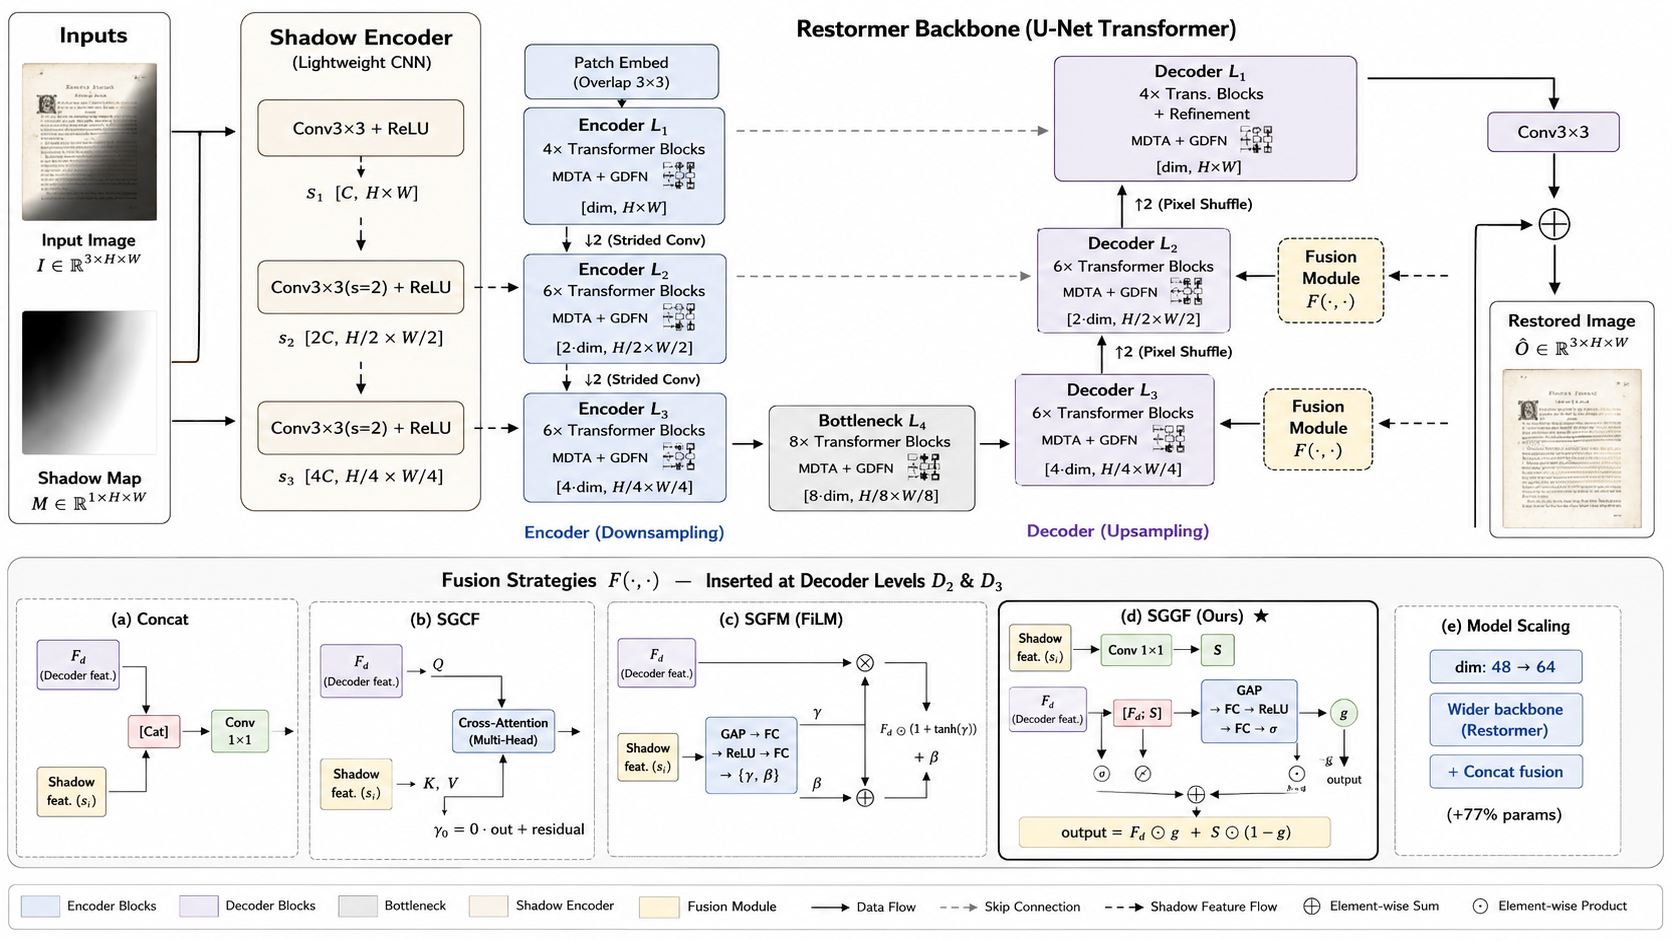
\includegraphics[width=0.95\textwidth]{fig1_overview.png}
\caption{Unified experimental framework. A Shadow Encoder extracts multi-scale features from the shadow prior, which are injected into the Restormer decoder through a Fusion Module. We evaluate five instantiations of the Fusion Module under identical training conditions across two datasets.}
\label{fig:overview}
\end{figure}

\subsection{Five Fusion Strategies}\label{sec:five_fusion}

Table~\ref{tab:fusion_overview} summarizes the five strategies, their key mechanisms, and the design rationale behind their inclusion.
Detailed formulations are provided in Appendix~\ref{sec:appendix_formulas}.

\begin{table}[t]
\caption{Five representative fusion strategies evaluated in this study. Parameter counts are for the Restormer dim=48 configuration.}
\label{tab:fusion_overview}
\begin{tabular}{@{}lllp{5.5cm}@{}}
\toprule
\textbf{Strategy} & \textbf{Type} & \textbf{Params} & \textbf{Design Rationale} \\
\midrule
Concat & Concatenation & +0.30M & Simplest baseline: let the network learn feature combination through subsequent convolutions. \\
Cross-Attn & Attention & +0.44M & Explicitly query shadow information via multi-head cross-attention with zero-initialized residual gating. \\
FiLM & Modulation & +0.34M & Lightweight channel-wise scaling and shifting: $F \odot (1+\tanh(\gamma)) + \beta$. \\
Gated & Gating & +0.29M & Sigmoid-gated convex combination $F \odot g + S \odot (1-g)$, avoiding $\tanh$ saturation. \\
Large & Capacity & +20.58M & No fusion design change; purely scale model width from dim=48 to dim=64. \\
\bottomrule
\end{tabular}
\end{table}

\textbf{Why these five.}
Concatenation serves as the minimal- complexity baseline.
Cross-Attention represents the pro-fusion position advocated by MDFormer~\cite{mdformer2025}.
FiLM is the most widely used lightweight modulation mechanism~\cite{perez2018film}, enabling us to test whether modulation-based fusion generalizes beyond synthetic domains.
The Gated strategy is motivated by our diagnostic findings: sigmoid gating with convex combination avoids the tanh saturation that destabilizes FiLM on real data.
The Large (capacity scaling) variant tests whether simply allocating more parameters to a simple fusion strategy can match the performance of complex fusion at lower capacity---a direct test of the ``fusion complexity vs.\ model capacity'' trade-off.

%%======================================================================%%
%%  4. Experiments                                                      %%
%%======================================================================%%
\section{Experiments}\label{sec:experiments}

\subsection{Experimental Setup}\label{sec:setup}

\textbf{Datasets.}
SD7K~\cite{li2023single} is a synthetic dataset containing 6,720 training pairs. For our controlled comparison, we sample a 200-pair subset and evaluate on the full 190-pair test set at 320$\times$320 resolution. This subset design is necessary because our experimental protocol requires training each fusion strategy on multiple subset sizes (30, 60, 100, 150, 200 pairs; Section~\ref{sec:scaling})---training all five strategies on the full 6,720 pairs would be computationally prohibitive. All models use the same 200-pair subset, ensuring fair comparison.
RDD is a real-world dataset with 1,080 training pairs at variable resolutions. We use 256$\times$256 random crops for training and evaluate on a held-out validation set.

\textbf{Training protocol.}
All models are trained for 200 epochs using AdamW ($\beta_1=0.9$, $\beta_2=0.999$, weight decay $10^{-4}$), initial learning rate $2\times10^{-4}$ halved at epochs 100 and 150, batch size 1 per GPU with gradient accumulation (2 steps).
All experiments run on 4$\times$NVIDIA RTX 3090 (24GB).
For FiLM on RDD, we additionally train a variant (v2) with gradient clipping at max\_norm=1.0 to diagnose the NaN instability.

\textbf{Metrics.}
We report PSNR, SSIM, RMSE, TextPSNR (PSNR computed exclusively on text regions detected by a pre-trained text detector), LPIPS~\cite{zhang2018lpips} (perceptual quality), inference time, and parameter count.

\subsection{Finding 1: Domain Flipping --- Synthetic vs.\ Real Optimal Strategies}\label{sec:main_results}

Table~\ref{tab:main_results} presents the main cross-domain comparison.

\begin{table}[t]
\caption{\textbf{Cross-domain comparison of fusion strategies.} All models use Restormer backbone, trained from scratch for 200 epochs. Bold = best. All RDD results at 320$\times$320 resolution unless noted. $\dagger$Cross-Attn at 192$\times$192 due to OOM; Gated at 256$\times$256. $^*$FiLM v2 with gradient clipping; v1 diverged to NaN at epoch 125/130 on RDD. Concat SSIM pending at 320$\times$320.}
\label{tab:main_results}
\footnotesize
\begin{tabular}{@{}lcccccc@{}}
\toprule
& \multicolumn{3}{c}{\textbf{SD7K (Synthetic)}} & \multicolumn{3}{c}{\textbf{RDD (Real)}} \\
\cmidrule{2-4}\cmidrule{5-7}
\textbf{Model} & \textbf{PSNR}$\uparrow$ & \textbf{SSIM}$\uparrow$ & \textbf{T-PSNR}$\uparrow$ & \textbf{PSNR}$\uparrow$ & \textbf{SSIM}$\uparrow$ & \textbf{T-PSNR}$\uparrow$ \\
\midrule
Restormer (no fusion) & 23.43 & 0.9174 & 26.62 & 35.72 & 0.9753 & 33.18 \\
Concat                & 23.74 & 0.9218 & 27.24 & \textbf{37.20} & -- & 34.52 \\
Cross-Attn            & 23.76 & 0.9164 & 26.46 & 37.03$^\dagger$ & 0.9701 & 32.92 \\
FiLM                  & \textbf{24.77} & \textbf{0.9308} & 27.47 & 37.01$^*$ & \textbf{0.9775} & 34.29 \\
Gated                 & 24.31 & 0.9243 & \textbf{27.75} & 35.53 & 0.9677 & 33.18 \\
Large                 & 24.51 & 0.9282 & 27.61 & 37.05 & 0.9749 & 33.49 \\
\bottomrule
\end{tabular}
\end{table}

\textbf{What this tells us.}
Three observations emerge:

\textit{(1) Domain-dependent ranking compression.}
On SD7K, FiLM opens a clear gap over the simplest baseline (+1.03~dB over Concat), demonstrating that complex modulation can exploit regular synthetic shadow patterns.
On RDD, however, the top four strategies (Concat, Large, Cross-Attn, FiLM) all fall within a narrow $\sim$0.2~dB band, with Concat marginally leading.
This is not a symmetric ``reversal'' but a pattern of \textit{ranking compression}: FiLM degrades on real data while Concat remains stable across both domains.
The practical implication is that complex fusion strategies are domain-sensitive, whereas simple concatenation is domain-robust.

\textit{(2) Theoretical validation.}
Cross-Attn provides only +0.02~dB over Concat on SD7K and underperforms by 0.21~dB on RDD---consistent with Zhou and Xie's~\cite{zhou2026feature} theoretical prediction that concatenation suffices when features are aligned in the representation space.

\textit{(3) Concatenation achieves the best TextPSNR on real data.}
On RDD, simple concatenation yields the highest TextPSNR (34.52~dB) among all configurations, including the fusion-free Restormer baseline (33.18~dB).
This reinforces the pattern: on real data, the simplest fusion mechanism provides the best all-around performance---best PSNR, best TextPSNR, and best perceptual quality (Section~\ref{sec:additional})---while complex modulation strategies offer no advantage for text preservation.

\subsection{Finding 2: Data Volume as Gap Modulator}\label{sec:scaling}

To disentangle the effects of data domain and data volume, we train three representative strategies (Concat, FiLM, Gated) on controlled SD7K subsets of 30, 60, 100, 150, and 200 training pairs.
Table~\ref{tab:scaling} and Figure~\ref{fig:scaling} present the results.

\begin{table}[t]
\caption{\textbf{Scaling curve on SD7K subsets.} PSNR reported on the SD7K test set. All models use dim=48. 30--150 pair subsets trained for 100 epochs; 200 pair subset uses the standard 200-epoch protocol.}
\label{tab:scaling}
\begin{tabular}{@{}lcccc@{}}
\toprule
\textbf{Data Pairs} & \textbf{Concat} & \textbf{FiLM} & \textbf{Gated} & \textbf{$\Delta$(FiLM$-$Concat)} \\
\midrule
30  & 22.98 & 23.35 & 23.31 & +0.37 \\
60  & 23.47 & 23.77 & 23.78 & +0.30 \\
100 & 23.56 & 23.93 & 23.31 & +0.37 \\
150 & 23.89 & 24.09 & 23.81 & +0.20 \\
200$^*$ & 23.74 & 24.77 & 24.31 & +1.03 \\
\bottomrule
\multicolumn{5}{l}{\small $^*$200 pairs trained for 200 epochs; other subsets trained for 100 epochs.} \\
\end{tabular}
\end{table}

\begin{figure}[t]
\centering
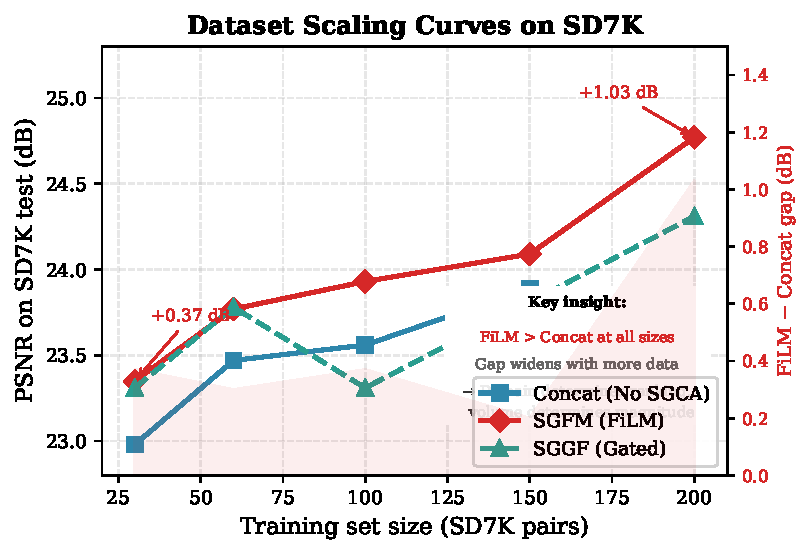
\includegraphics[width=0.85\textwidth]{fig_scaling_curve.pdf}
\caption{Scaling behavior of three fusion strategies on SD7K subsets. FiLM maintains consistent superiority across all data volumes; the gap widens with more data. No crossover point is observed.}
\label{fig:scaling}
\end{figure}

\textbf{What this tells us.}
FiLM outperforms Concat at \textit{all} data volumes---there is no crossover point.
The domain (synthetic) fixes the ranking; additional data amplifies the advantage from +0.37~dB (30 pairs) to +1.03~dB (200 pairs).
This establishes the \textbf{dual constraint law}: \textit{data domain determines which strategy ranks highest; data volume determines the magnitude of the performance gap.}
For practitioners, this means that when domain characteristics are unknown, the safe default is the simplest strategy; when the domain is well-characterized (e.g., synthetic with regular patterns), investing in complex fusion yields returns proportional to available data.

\subsection{Finding 3: Self-Attention as Built-in Cross-Modal Interaction}\label{sec:attention}

To understand \textit{why} complex fusion provides such limited benefit over concatenation, we visualize the decoder self-attention maps from Restormer's Level~3 (deepest decoder layer).
Figure~\ref{fig:attention} overlays attention weights on input images for four configurations: Restormer baseline (no fusion), Concat, FiLM, and Gated.

\begin{figure}[t]
\centering
\includegraphics[width=0.95\textwidth]{fig_attention_viz.pdf}
\caption{Decoder self-attention visualization at Level~3. Even without any shadow encoder or fusion module (\textbf{leftmost column}), Restormer's self-attention already focuses on shadow regions (highlighted in red). Models with fusion exhibit attention patterns strikingly similar to the baseline---fusion enhances rather than establishes cross-modal attention.}
\label{fig:attention}
\end{figure}

\textbf{What this tells us.}
Three observations are evident:
(1)~The Restormer baseline, which has no shadow encoder and therefore no explicit shadow information, already directs self-attention toward shadow regions.
This occurs because skip connections feed encoder features directly to the decoder, where self-attention operates over the joint set of encoder and decoder tokens, naturally learning to attend to shadow-affected areas.
(2)~Models with fusion modules (Concat, FiLM, Gated) produce attention patterns highly similar to the baseline---fusion \textit{enhances} existing attention rather than \textit{establishing} new cross-modal connections.
(3)~This directly explains why Cross-Attn yields negligible gains: the decoder's self-attention has already performed the cross-modal alignment that explicit cross-attention aims to provide.
These findings provide the first direct visual evidence supporting Zhou and Xie's theoretical prediction~\cite{zhou2026feature} and extend its applicability: any Transformer U-Net with self-attention on skip connections will exhibit this built-in alignment property.

\subsection{Finding 4: Generalization and Fine-tuning Reveal Robustness Differences}\label{sec:generalization}

\textbf{Cross-domain generalization.}
Table~\ref{tab:cross_domain} reports zero-shot cross-domain transfer.

\begin{table}[t]
\caption{\textbf{Cross-domain generalization.} Models trained on one domain, evaluated on the other without fine-tuning. The domain gap is strongly asymmetric. Bold = best in each transfer direction.}
\label{tab:cross_domain}
\begin{tabular}{@{}lcccc@{}}
\toprule
\textbf{Model} & \textbf{Train}$\rightarrow$Test & \textbf{PSNR}$\uparrow$ & \textbf{SSIM}$\uparrow$ \\
\midrule
Cross-Attn & RDD$\rightarrow$SD7K & 14.60 & 0.457 \\
Large      & RDD$\rightarrow$SD7K & 14.72 & 0.459 \\
\midrule
Restormer   & SD7K$\rightarrow$RDD & 17.29 & 0.848 \\
Concat      & SD7K$\rightarrow$RDD & \textbf{18.59} & 0.867 \\
FiLM        & SD7K$\rightarrow$RDD & 18.26 & \textbf{0.892} \\
Gated       & SD7K$\rightarrow$RDD & 18.25 & 0.870 \\
Large       & SD7K$\rightarrow$RDD & 17.78 & 0.858 \\
GatedLarge  & SD7K$\rightarrow$RDD & 17.77 & 0.870 \\
\bottomrule
\end{tabular}
\end{table}

Two patterns emerge. First, a \textbf{strongly asymmetric domain gap}: RDD$\rightarrow$SD7K transfer is catastrophic ($\sim$14.6~dB), while SD7K$\rightarrow$RDD achieves partial transfer ($\sim$18.6~dB)---a $\sim$4~dB asymmetry.
Second, \textbf{Concat is the best zero-shot generalizer} in the practically relevant synthetic-to-real direction (18.59~dB), and larger models (Large, GatedLarge at dim=64) generalize \textit{worse} than their dim=48 counterparts, indicating that increased capacity amplifies overfitting to synthetic domain artifacts.

\textbf{Fine-tuning analysis.}
Table~\ref{tab:finetune} reports SD7K-pretrained models fine-tuned on RDD for 200 epochs.

\begin{table}[t]
\caption{\textbf{SD7K$\rightarrow$RDD fine-tuning.} All models pre-trained on SD7K (200 epochs), then fine-tuned on RDD (200 epochs, lr=$1\times10^{-4}$).}
\label{tab:finetune}
\begin{tabular}{@{}lcccc@{}}
\toprule
\textbf{Model} & \textbf{Scratch PSNR} & \textbf{Finetune PSNR} & \textbf{$\Delta$} & \textbf{Status} \\
\midrule
Gated   & 35.53 & 36.97 & \textbf{+1.44} & Stable \\
Large   & 37.05 & 36.39 & --0.66 & Degraded \\
FiLM    & 37.01 & NaN   & --    & Collapsed (E40) \\
\bottomrule
\end{tabular}
\end{table}

\textbf{What this tells us.}
Pre-training is not a universal remedy; its effect depends on the fusion mechanism.
The Gated strategy benefits most (+1.44~dB), suggesting that sigmoid gating benefits from synthetic pre-training to learn initial shadow representations before adapting to real data.
Large models degrade (--0.66~dB), consistent with pre-training steering the larger capacity toward a synthetic-domain local optimum from which fine-tuning cannot escape from with limited real data.
Critically, \textbf{FiLM collapses to NaN at epoch 40 even with pre-training}, confirming that its tanh saturation instability is a mechanism-level property that cannot be resolved by better initialization alone.

\subsection{Additional Analyses}\label{sec:additional}

\textbf{FiLM collapse root cause.}
We diagnose FiLM's NaN divergence through gradient statistics analysis (Figure~\ref{fig:film}).
When tanh saturates at $\pm1$, its derivative approaches zero, creating a gradient dead zone that simultaneously affects all pathways through the modulated features.
Unlike ReLU-based networks where non-zero gradient paths always exist, tanh saturation creates an inescapable region for the optimizer.
This occurs on RDD (three independent runs: epochs 125, 130, and 30 during fine-tuning) but not on SD7K, because real-world shadows require larger modulation values that push tanh into saturation.
Gradient clipping (max\_norm=1.0) rescues training, confirming the failure is optimization-level (unconstrained gradients through saturating nonlinearities) rather than architecture-level.

\begin{figure}[t]
\centering
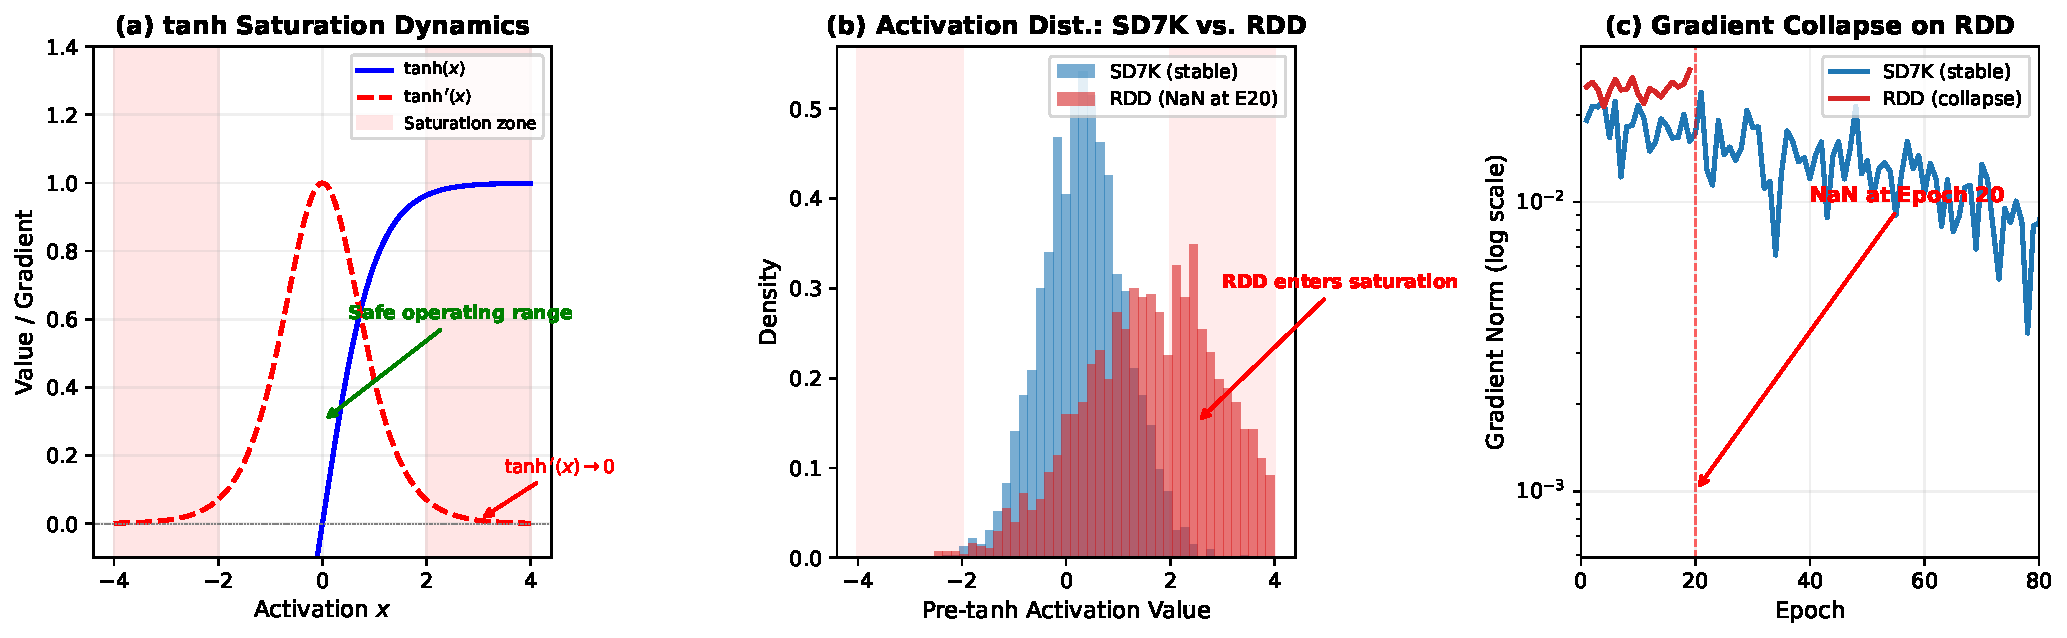
\includegraphics[width=0.85\textwidth]{fig_film_analysis.pdf}
\caption{FiLM gradient dynamics on RDD. tanh saturation causes gradient vanishing in the modulation pathway, triggering NaN divergence. Gradient clipping prevents saturation by bounding gradient magnitudes.}
\label{fig:film}
\end{figure}

\textbf{Ablation study.}
Removing the shadow encoder (zero shadow input) decreases PSNR by 0.19~dB (24.12 vs.\ 24.31 for Gated), confirming that the shadow prior provides non-trivial complementary information.
Restricting fusion to a single decoder level (Level~3 only) costs 0.37~dB (23.94 vs.\ 24.31), validating the value of multi-scale fusion at complementary spatial granularities.

\textbf{Perceptual quality and efficiency.}
Table~\ref{tab:supplementary} consolidates perceptual quality (LPIPS), OCR recovery rate, and computational efficiency.
A striking dissociation emerges: Concat achieves the best LPIPS (0.0461) despite being the simplest method, while FiLM---the PSNR leader on SD7K (24.77~dB)---records the \textit{worst} LPIPS (0.0557) among dim=48 models, even trailing the fusion-free Restormer baseline (0.0554).
This PSNR-perceptual trade-off reveals that FiLM's aggressive channel-wise modulation introduces subtle artifacts perceptible to humans.
OCR recovery rates are uniformly high across all models ($\geq$98.1\%), confirming that shadow removal substantially improves downstream text recognition regardless of the fusion strategy employed.
Cross-Attn incurs a 4$\times$ memory overhead (2,774~MB at 192$\times$192 vs.\ $\sim$699~MB for other methods at 256$\times$256), making it impractical for high-resolution document processing.

\begin{table}[t]
\caption{\textbf{Supplementary metrics.} LPIPS (lower is better), OCR recovery rate, and efficiency. All measurements at training resolution on RTX 3090. $\dagger$Cross-Attn evaluated at 192$\times$192 due to OOM at higher resolutions.}
\label{tab:supplementary}
\footnotesize
\begin{tabular}{@{}lccccc@{}}
\toprule
\textbf{Model} & \textbf{LPIPS}$\downarrow$ & \textbf{OCR}$\uparrow$ & \textbf{Param (M)} & \textbf{Time (ms)} & \textbf{Mem (MB)} \\
\midrule
Restormer  & 0.0554 & 98.1\%  & 26.13 & 181.6 & 676 \\
Concat     & \textbf{0.0461} & 98.6\%  & 26.43 & 181.9 & 699 \\
Cross-Attn & 0.0480 & 81.9\%$^\dagger$ & 26.57 & 135.0 & 2774 \\
FiLM       & 0.0557 & \textbf{101.3\%} & 26.47 & 182.5 & 699 \\
Gated      & 0.0496 & 100.2\% & 26.42 & 182.6 & 699 \\
Large      & 0.0496 & 99.6\%  & 46.71 & 346.0 & 1418 \\
\bottomrule
\end{tabular}
\end{table}

\textbf{Extended training.}
All models trained beyond 200 epochs exhibit mild overfitting (400-epoch PSNR drops: Gated 24.31$\rightarrow$24.18, Large 24.51$\rightarrow$24.29, FiLM 24.77$\rightarrow$24.63), establishing 200 epochs as the optimal stopping point for SD7K-scale data.

%%======================================================================%%
%%  5. Discussion                                                       %%
%%======================================================================%%
\section{Discussion}\label{sec:discussion}

\subsection{Why Features Are Already Aligned in Restormer}

The attention visualization results (Section~\ref{sec:attention}) raise a natural question: what mechanism enables Restormer to align multi-modal features without explicit fusion?
The answer lies in the interaction between skip connections and Transformer self-attention.
In Restormer's U-Net architecture, skip connections concatenate encoder features directly with decoder features at each resolution level.
The decoder's MDTA (multi-dconv head transposed attention) then computes self-attention over this joint set of tokens.
Since attention weights are computed from pairwise token interactions, the encoder tokens and decoder tokens attend to each other through the same softmax operation, producing implicit cross-modal alignment as a by-product of self-attention.
This is not unique to Restormer---any Transformer U-Net with self-attention on skip-connected features will exhibit this property, including SwinIR and Uformer.
The practical implication is that for such architectures, the default fusion strategy should be the simplest one (concatenation), with complexity added only when domain analysis suggests untapped modulation potential.

\subsection{Reconciling the Fusion Debate}

Our results provide a unified explanation for the conflicting claims in the fusion literature (Section~\ref{sec:debate}):

\begin{center}
\footnotesize
\begin{tabular}{@{}p{3.8cm}p{3.5cm}p{4.5cm}@{}}
\toprule
\textbf{Condition} & \textbf{Prediction} & \textbf{Evidence} \\
\midrule
Backbone has self-attn + skip conn. & Features aligned $\rightarrow$ Concat suffices & This work + Zhou \& Xie~\cite{zhou2026feature} \\
Backbone lacks this mechanism & Features unaligned $\rightarrow$ Dedicated fusion needed & MDFormer~\cite{mdformer2025}, RadFuse~\cite{radfuse2025} \\
\bottomrule
\end{tabular}
\end{center}

The contradiction is not about who is right or wrong, but about \textbf{conditions}.
Works supporting dedicated fusion typically employ backbones without Transformer self-attention on skip connections, where explicit cross-modal interaction must be provided by the fusion module.
Works finding fusion redundancy employ architectures where self-attention already provides this interaction.
Our direct evidence---attention visualization plus controlled cross-domain experiments---closes the loop between theory~\cite{zhou2026feature} and practice.

\subsection{The Boundary: Why FiLM Wins on Synthetic but Collapses on Real}

FiLM's domain-dependent behavior---best PSNR on SD7K, catastrophic NaN on RDD---reveals an important boundary condition for modulation-based fusion.
Synthetic shadows follow regular, procedurally generated patterns.
FiLM's per-channel scaling and shifting can learn to amplify channels sensitive to these predictable patterns and suppress others, effectively learning a specialized shadow detector.
Real-world shadows, by contrast, are irregular, overlapping, and influenced by complex illumination interactions.
The tanh-bounded modulation parameters cannot find stable values for such diverse inputs, oscillate toward saturation, and trigger gradient collapse.
\textbf{The ceiling of modulation-based fusion is determined by the learnability of domain features.}
When the domain exhibits regular structure amenable to parametric modulation, FiLM excels; when the domain is inherently irregular, modulation becomes a liability.

\subsection{Practical Recommendations}

Based on our findings, we propose a decision framework for fusion strategy selection (Figure~\ref{fig:decision}):

\begin{figure}[t]
\centering
\begin{tabular}{@{}p{0.95\textwidth}@{}}
\toprule
\textbf{Decision Framework for Fusion Strategy Selection} \\
\midrule
\textbf{Q1:} Does the backbone have self-attention operating on skip-connected features? \\
\quad $\rightarrow$ \textbf{No}: Dedicated fusion is necessary. Choose Cross-Attn or Gated based on data volume. \\
\quad $\rightarrow$ \textbf{Yes}: Proceed to Q2. \\
\textbf{Q2:} Is the training data synthetic or real? \\
\quad $\rightarrow$ \textbf{Synthetic}: Proceed to Q3. \\
\quad $\rightarrow$ \textbf{Real}: Proceed to Q4. \\
\textbf{Q3:} How many training pairs are available? \\
\quad $\rightarrow$ \textbf{$<$100 pairs}: Use Gated (better text preservation at low data). \\
\quad $\rightarrow$ \textbf{$>$150 pairs}: Use FiLM + gradient clipping (best PSNR; monitor training stability). \\
\textbf{Q4:} What is the primary deployment objective? \\
\quad $\rightarrow$ \textbf{Stability and robustness}: Use Concat (default first choice; best zero-shot generalization). \\
\quad $\rightarrow$ \textbf{Maximum performance}: Use Large (dimension scaling provides safe gains without mechanism risk). \\
\quad $\rightarrow$ \textbf{Text preservation}: Use Concat (best TextPSNR 34.52~dB on RDD; see Table~\ref{tab:main_results}). \\
\bottomrule
\end{tabular}
\caption{Decision framework for selecting fusion strategies based on backbone architecture, data domain, data volume, and deployment objectives.}
\label{fig:decision}
\end{figure}

This framework is offered as a starting point for practitioners, grounded in the evidence from our controlled study, rather than as a universal prescription.

\subsection{Limitations}

Our study has four main limitations that define directions for future work:

\begin{enumerate}
  \item \textbf{Single backbone validation.} All experiments use Restormer as the backbone. While we argue that the underlying mechanism (self-attention on skip connections) generalizes to other Transformer U-Nets (SwinIR, Uformer), empirical verification across architectures is needed.
  \item \textbf{Limited real-world data.} RDD contains 1,080 training pairs. Larger-scale real-world datasets, if available, could shift the conclusions---particularly whether FiLM's instability persists or can be overcome with sufficient diverse real data.
  \item \textbf{Two-domain coverage.} Our study spans synthetic (SD7K) and real (RDD) document shadows. Extension to other domains (natural image restoration, medical imaging) would test whether the domain-dependent ranking pattern generalizes.
  \item \textbf{Empirical rather than theoretical analysis.} Our characterization of fusion behavior is based on controlled experimentation. A rigorous sample-complexity analysis for modulation-based fusion, analogous to Zhou and Xie's~\cite{zhou2026feature} analysis of cross-attention vs.\ concatenation, remains open.
\end{enumerate}

%%======================================================================%%
%%  6. Conclusion                                                       %%
%%======================================================================%%
\section{Conclusion}\label{sec:conclusion}

We presented a systematic characterization of feature fusion strategies in Transformer-based image restoration.
Through controlled experiments spanning five fusion strategies, two datasets, and multi-dimensional analysis including scaling curves, attention visualization, and cross-domain evaluation, we established three findings: (1)~Transformer self-attention on skip connections already provides implicit cross-modal alignment, making lightweight fusion sufficient; (2)~the optimal fusion strategy depends on data domain, with data volume modulating the performance gap; and (3)~FiLM modulation carries a mechanism-level instability risk on real-world data that requires active gradient management.
These findings reconcile the ongoing debate between fusion advocates and fusion skeptics by identifying backbone architecture as the critical conditioning variable.
More broadly, our work demonstrates that diagnostic evaluation---understanding \textit{why} and \textit{when} methods succeed or fail---yields actionable knowledge that benchmark-driven comparisons cannot provide.
The decision framework we derived offers practitioners evidence-based guidance for fusion strategy selection, and the diagnostic methodology we employed provides a template for analogous investigations in other guided image restoration tasks.

%%======================================================================%%
%%  Declarations                                                        %%
%%======================================================================%%
\backmatter

\bmhead{Acknowledgments}
This work was supported by [funding information to be added].

\section*{Declarations}

\begin{itemize}
  \item \textbf{Funding}: [to be added]
  \item \textbf{Conflict of interest}: The authors declare no competing interests.
  \item \textbf{Ethics approval}: Not applicable.
  \item \textbf{Data availability}: The SD7K dataset is publicly available. The RDD dataset is available from the corresponding author upon reasonable request.
  \item \textbf{Code availability}: Code will be released upon acceptance.
  \item \textbf{Author contribution}: All authors contributed to the study design, experimental execution, and manuscript preparation.
\end{itemize}

%%======================================================================%%
%%  Appendix: Detailed Fusion Formulations                               %%
%%======================================================================%%
\begin{appendices}

\section{Detailed Fusion Strategy Formulations}\label{sec:appendix_formulas}

Let $\mathbf{F}_d \in \mathbb{R}^{C_d \times H \times W}$ denote decoder features and $\mathbf{F}_s \in \mathbb{R}^{C_s \times H \times W}$ denote shadow encoder features at the same spatial resolution.
We define the five fusion operations below.

\subsection*{Concatenation (Concat)}
\begin{equation}
  \mathbf{F}_{\text{out}} = \text{Conv}_{1\times1}\big([\,\mathbf{F}_d \,;\, \text{Proj}(\mathbf{F}_s)\,]\big)
\end{equation}
Shadow features are projected via $1\times1$ convolution to match the decoder channel dimension, then concatenated along the channel axis and reduced back to $C_d$ channels.

\subsection*{Cross-Attention (Cross-Attn)}
\begin{equation}
  \mathbf{Q} = \mathbf{W}_q(\mathbf{F}_d), \quad \mathbf{K} = \mathbf{W}_k(\mathbf{F}_s), \quad \mathbf{V} = \mathbf{W}_v(\mathbf{F}_s)
\end{equation}
\begin{equation}
  \mathbf{F}_{\text{attn}} = \text{Softmax}\!\left(\frac{\mathbf{Q}\mathbf{K}^\top}{\sqrt{d_k}}\right)\mathbf{V}
\end{equation}
\begin{equation}
  \mathbf{F}_{\text{out}} = \mathbf{F}_d + \gamma \cdot \mathbf{W}_o(\mathbf{F}_{\text{attn}})
\end{equation}
Multi-head cross-attention (4 heads) with zero-initialized learnable gating parameter $\gamma$.

\subsection*{FiLM Modulation}
\begin{equation}
  \gamma(\mathbf{F}_s),\; \beta(\mathbf{F}_s) = \text{Split}\big(\text{GAP}(\mathbf{F}_s) \rightarrow \text{FC} \rightarrow \text{FC}\big)
\end{equation}
\begin{equation}
  \mathbf{F}_{\text{out}} = \mathbf{F}_d \odot \big(1 + \tanh(\gamma)\big) \;+\; \beta
\end{equation}
Global average pooling followed by a two-layer MLP predicts channel-wise modulation parameters.

\subsection*{Gated Fusion}
\begin{equation}
  \mathbf{S} = \text{Conv}_{1\times1}(\mathbf{F}_s)
\end{equation}
\begin{equation}
  \mathbf{g} = \sigma\big(\text{FC}_2(\text{ReLU}(\text{FC}_1(\text{GAP}([\mathbf{F}_d; \mathbf{S}]))))\big) \in \mathbb{R}^{C_d \times 1 \times 1}
\end{equation}
\begin{equation}
  \mathbf{F}_{\text{out}} = \mathbf{F}_d \odot \mathbf{g} \;+\; \mathbf{S} \odot (1 - \mathbf{g})
\end{equation}
Sigmoid gating with a bottleneck structure (compression ratio 4). The convex combination guarantees $\mathbf{F}_{\text{out}}$ is always bounded.

\subsection*{Capacity Scaling (Large)}
Identical to Concatenation, but with the Restormer backbone width expanded from dim=48 to dim=64, unified across all components (encoder, decoder, shadow encoder, fusion projection).

\end{appendices}

%%======================================================================%%
%%  Bibliography                                                        %%
%%======================================================================%%
\bibliography{sn-bibliography}

\end{document}
